\documentclass[tikz,border=2pt]{standalone}
\usepackage{amsmath,amssymb}
\usepackage{pgfplots}
\pgfplotsset{compat=1.18}

\begin{document}
% Joint density 2 on the triangle 0 < y < x < 1. Given X = x, Y is uniform on (0, x); its mean
% x/2 traces the line g(x) = x/2, and E[Y | X] = g(X) is a random variable.
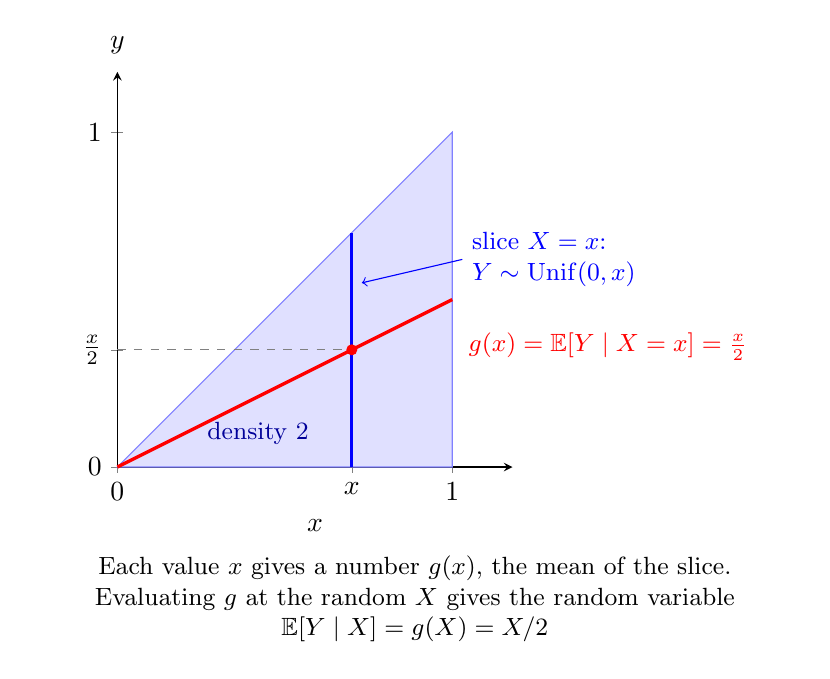
\begin{tikzpicture}
	\begin{axis}[
		axis lines=left, xmin=0, xmax=1.18, ymin=0, ymax=1.18,
		xtick={0,0.7,1}, xticklabels={$0$,$x$,$1$}, ytick={0,0.35,1}, yticklabels={$0$,$\tfrac x2$,$1$},
		xlabel={$x$}, ylabel={$y$}, ylabel style={rotate=-90, anchor=south, at={(axis description cs:0,1.02)}},
		width=6.6cm, height=6.6cm, clip=false
		]
		\addplot[fill=blue!12, draw=blue!50] coordinates {(0,0) (1,0) (1,1)} -- cycle;
		\draw[blue, very thick] (axis cs:0.7,0) -- (axis cs:0.7,0.7);
		\addplot[red, very thick, domain=0:1] {x/2};
		\draw[gray, dashed] (axis cs:0,0.35) -- (axis cs:0.7,0.35);
		\fill[red] (axis cs:0.7,0.35) circle (2pt);
		\node[blue!60!black, font=\small] at (axis cs:0.42,0.1) {density $2$};
		\node[blue, anchor=west, font=\small, align=left] at (axis cs:1.03,0.62) {slice $X=x$:\\ $Y\sim\operatorname{Unif}(0,x)$};
		\draw[blue, ->] (axis cs:1.03,0.62) -- (axis cs:0.73,0.55);
		\node[red, anchor=west, font=\small] at (axis cs:1.02,0.36) {$g(x)=\mathbb{E}[Y\mid X=x]=\tfrac x2$};
	\end{axis}
	\node[anchor=north, font=\small, align=flush center, text width=9.6cm] at ([yshift=-2pt]current axis.outer south) {Each value $x$ gives a number $g(x)$, the mean of the slice. Evaluating $g$ at the random $X$ gives the random variable $\mathbb{E}[Y\mid X]=g(X)=X/2$};
\end{tikzpicture}
\end{document}
